% Chapter Template

\chapter{Ensayos y resultados} % Main chapter title

\label{Chapter4} % Change X to a consecutive number; for referencing this chapter elsewhere, use \ref{ChapterX}

%----------------------------------------------------------------------------------------
%	SECTION 1
%----------------------------------------------------------------------------------------

\section{Pruebas funcionales de hardware y rediseño}
%\label{sec:pruebasHW}

En el presente capítulo se explican los ensayos realizados sobre el prototipo de equipo dip coater, se presentan y analizan los resultados obtenidos y se analizan futuros cambios.
\subsection{Comunicación con periféricos}

\subsection{Ensayo de funcionamiento}

\section{Pruebas funcionales firmware y rediseño}
\subsection{Tiempo de ejecución de movimientos}

El ensayo se realizo para verificar los parámetros que definen el desplazamiento de la muestra, es decir para verificar que las velocidades y aceleraciones que definen movimientos sean similares a las que surgen del cálculo teórico.
En el capítulo \ref{Chapter3} se detalló la configuración de la rampa de seis puntos que define un movimiento y se mostró como se configuraron los parámetros para obtener una rampa de cuatro puntos en donde la rampa de aceleración es igual a la rampa de desaceleración.

Dicha rampa esta definida por la siguiente ecuación \ref{eq:movimiento_completo}.

\begin{equation}
	\label{eq:movimiento_completo}
	\vec{x}=\vec{x_o}+\vec{v}(t-t_o)+\frac12 \vec {a} (t-t_o)^2
\end{equation}
%(((2*velocidad)/(aceleración*1000))+(desplazamiento/velocidad))*60*1000  

Por lo tanto, con los valores de aceleración, desaceleración, velocidad y desplazamiento se puede calcular el tiempo teórico necesario para la ejecución de un movimiento.
A continuación en la siguiente tabla se observan los valores de los parámetros ensayados.

\begin{table}[h]
	\centering
	\caption[Ensayo de tiempo en desplazamientos]{Ensayo de tiempos en desplazamiento}
	\begin{tabular}{c c c }    
		\toprule
		\textbf{Velocidad (mm/min)}     & \textbf{Aceleración-Desaceleración(m/min)} & \textbf{Desplazamiento(mm)} \\
		\midrule
		1  mm/min	 & 	   100-500-1000-2100 m/min2     & 	50 mm 			 	\\		
		10  mm/min   & 	   100-500-1000-2100 m/min2 	& 	50 mm				\\
		100  mm/min  & 	   100-500-1000-2100 m/min2	    & 	50 mm 				\\
		200  mm/min	 & 	   100-500-1000-2100 m/min2	    & 	50 mm 			\\
		500  mm/min	 & 	   100-500-1000-2100 m/min2     & 	50 mm					\\
		800  mm/min	 & 	   100-500-1000-2100 m/min2     & 	50 mm					\\
		\bottomrule
		\hline
	\end{tabular}
	\label{tab:ensayo_comandos}
\end{table}

Para realizar el ensayo se preparo un bloque de código que funciono de la siguiente manera:

\begin{enumerate}
\item Se configura un movimiento descendente con los parámetros ya mencionados.
\item Se ejecuta el movimiento, al iniciar se registra el tiempo del sistema.
\item Al terminar el movimiento, se registra el tiempo del sistema, se calcula el tiempo que llevo dicho movimiento, se envía por terminal UART un bloque con toda la información.
\item Se pasa al siguiente parámetro y se repite el ciclo.
\item El ordenador conectado al equipo ejecuta un script de Python que almacena los datos recibidos en un archivo.
\end{enumerate}


\begin{figure}[h]
\centering 
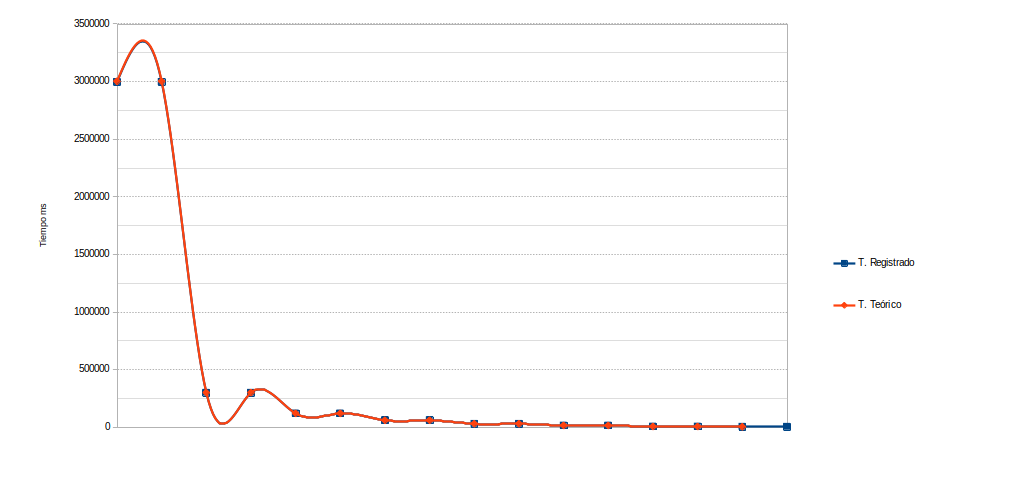
\includegraphics[width=1.2\textwidth]{./Figures/tiempo_movimiento_1.png}
\caption{Comparación de tiempos teóricos y registrados.}
\end{figure}



  
\section{Calibración del equipo}
\label{sec:calibración}
\subsection{Desplazamiento lineal y micro pasos}

Este ensayo se realizo para definir y ajustar la constante de desplazamiento que relaciona los micros pasos realizados por el motor con la distancia de desplazamiento del carro. La misma es una constante que queda definida por las dimensiones del tornillo, es decir el paso del mismo,  sobre el cual de desplaza el carro.

Para realizar las mediciones se utilizó un comparador digital de la marca Asimeto\citep{web_asimeto} el cual puede observarse en la figura \ref{fig:micrometro}, el mismo tiene una resolución de 0.0001 mm y permite desplazamientos de 0 a 50 mm.


\begin{figure}[h]
\centering 
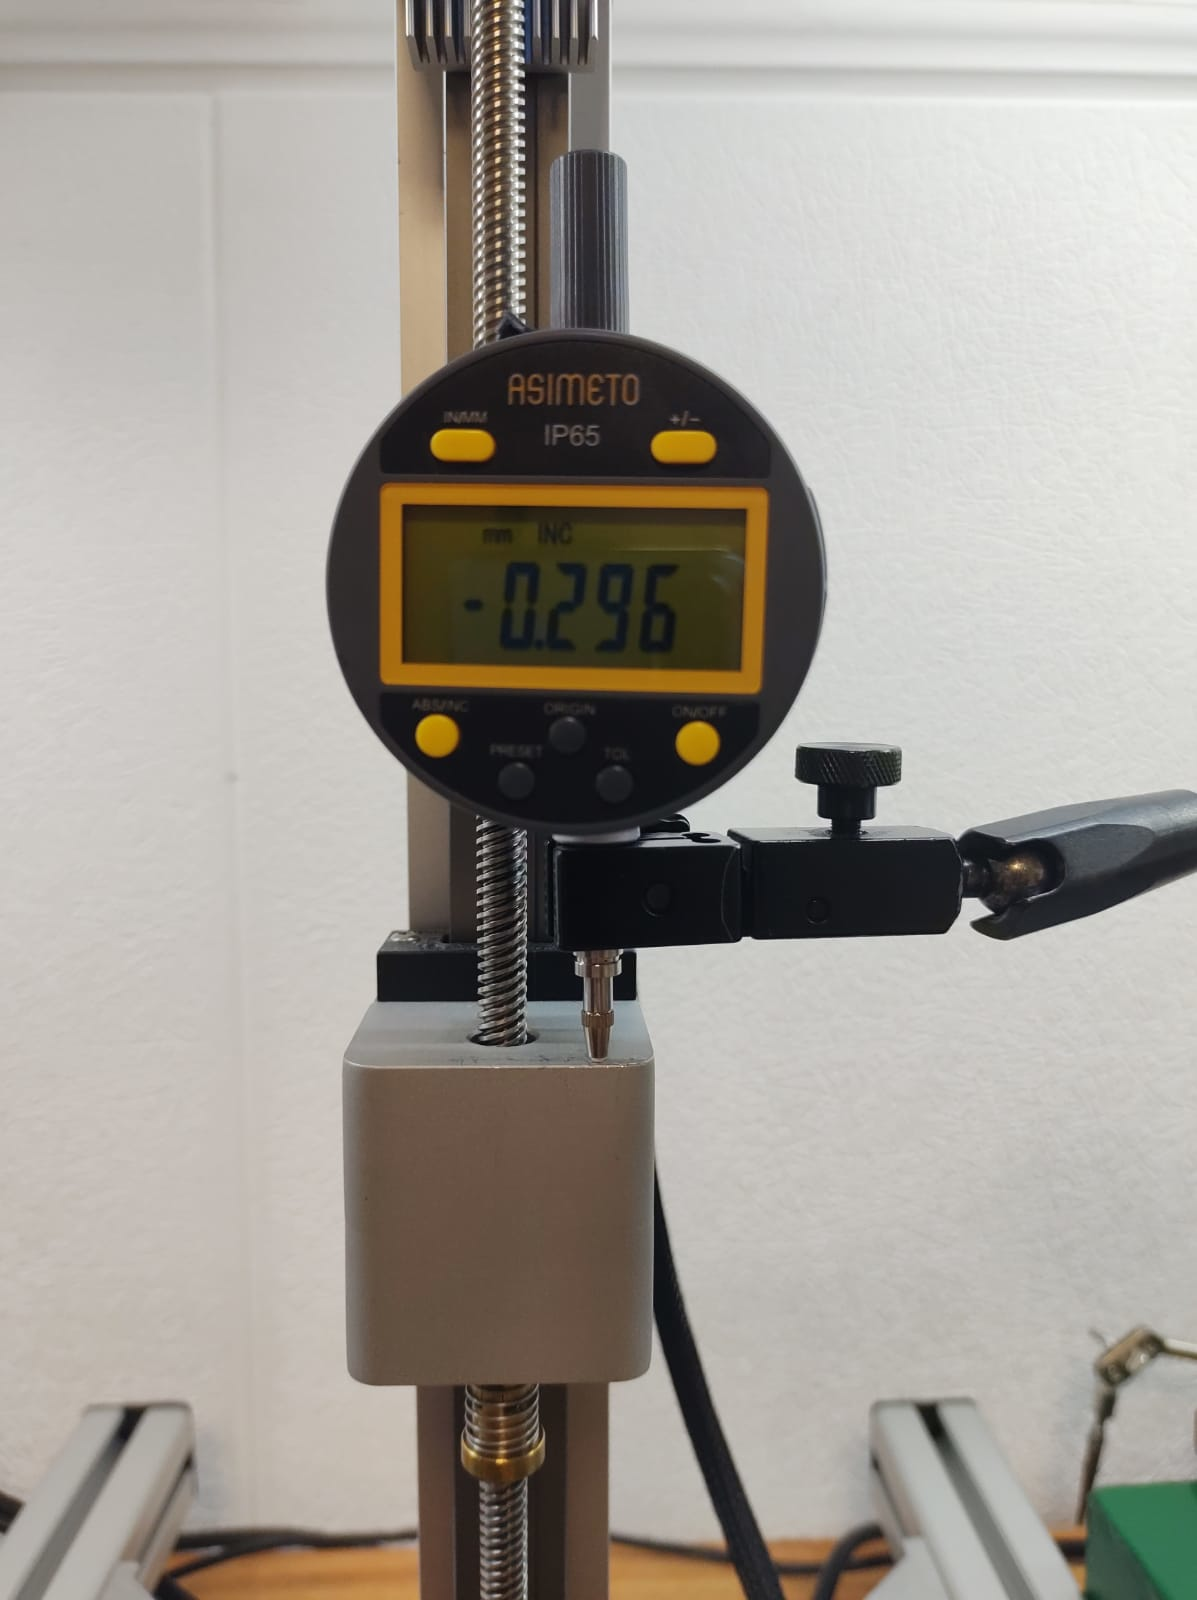
\includegraphics[width=0.5\textwidth]{./Figures/micrometro.png}
\caption{Comparador digital Asimeto.}
\label{fig:micrometro}
\end{figure}

El ensayo consistió en medir seis desplazamientos sucesivos de 1 mm sobre el carro de manera descendente y luego de manera ascendente. Este ensayo en muy importante porque permite corregir la unidad de conversión de micro pasos a milímetros que utiliza el CI TMC5130 para realizar todos los movimientos. 
En la subsección \ref{subsec:calibracion} se mencionó la macro \textit{MACHINE STEPS PER MILLIMETER} definida en el archivo hardware.h que surgió de este ensayo. 

En la figura \ref{fig:desplazamiento_lineal} se observa el banco de medición donde se visualiza el comparador Asimeto apoyado sobre una base metálica independiente al equipo dip coater con la punta del mismo en contacto directo con el carro de desplazamiento.

\begin{figure}[h]
\centering 
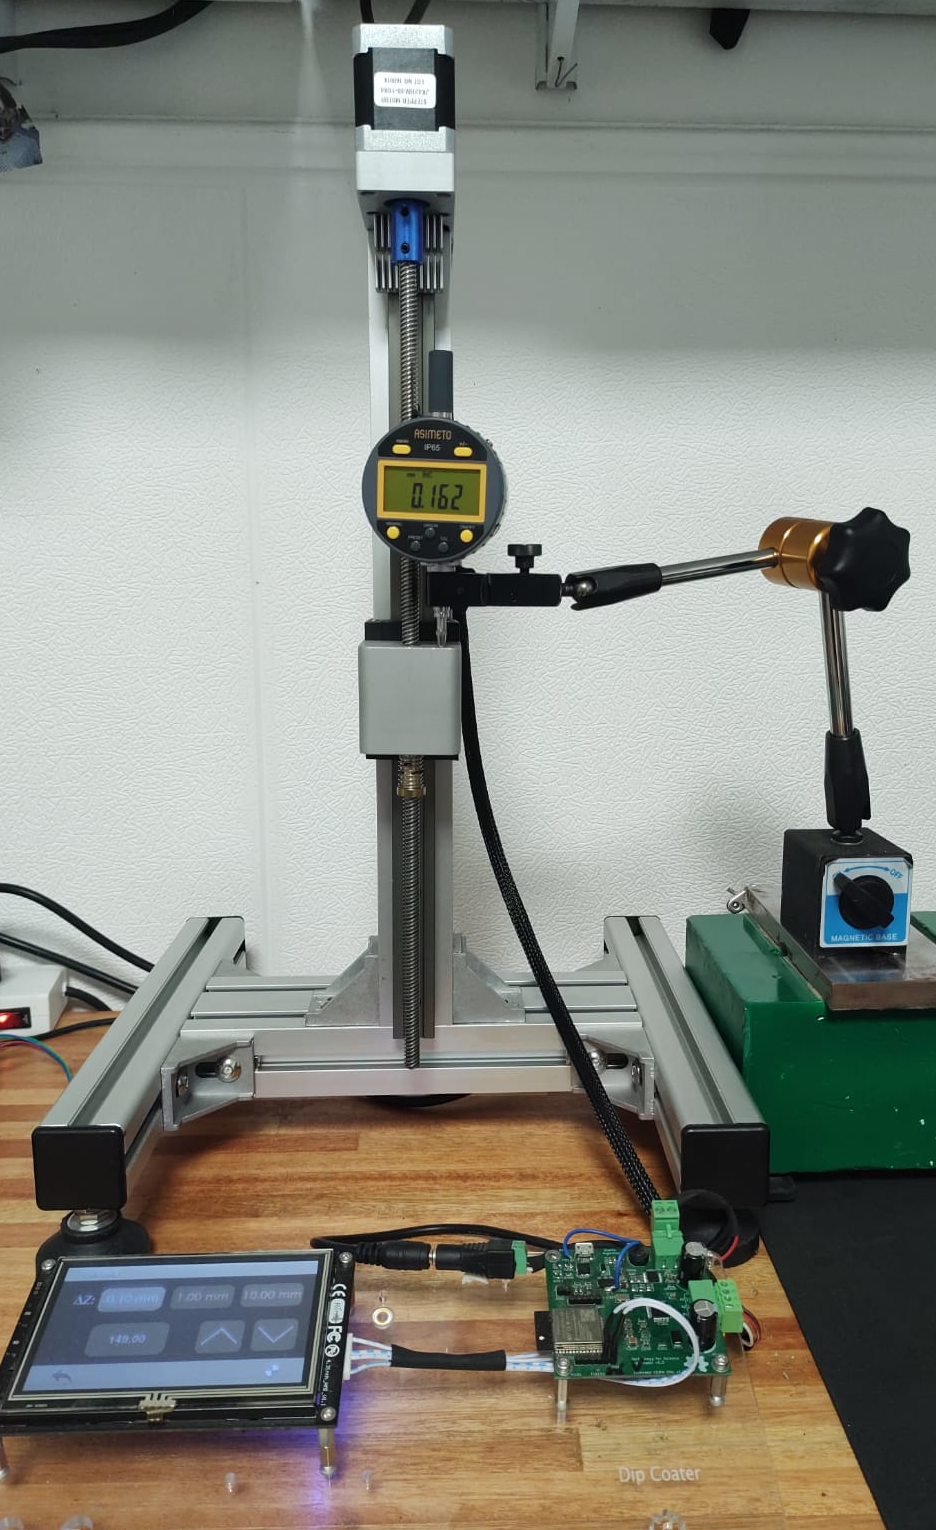
\includegraphics[width=0.5\textwidth]{./Figures/desplazamiento_lineal.png}
\caption{Ensayo de desplazamiento lineal.}
\label{fig:desplazamiento_lineal}
\end{figure}


Para iniciar el ensayo se presiona el botón \textit{origin} en el comparador para poner en cero la medida, la sensibilidad del mismo es tan grande que es difícil dejar la medida inicial en 0,000 mm debido  a la acción de apretar el botón. Luego se realizan movimientos descendentes de 1 mm y se registran en la siguiente tabla \ref{tab:ensayo_desplazamiento_}.

\begin{table}[h]
	\centering
	\caption[Ensayo de desplazamiento]{Ensayo de desplazamiento lineal descendentes}
	\begin{tabular}{l c c }    
		\toprule
		\textbf{Posición absoluta}     & \textbf{Desplazamiento relativo} & \textbf{Error Relativo} \\
		\midrule
		0,058 mm	& 	        	& 	 			 	\\		
		1,051 mm    & 	0,993 mm    	& 	0,007				\\
		2,035 mm 	& 	0,984 mm	    & 	0,016 				\\
		3,034 mm	& 	0,999 mm	    & 	0,001 			\\
		4,054 mm 	& 	1,02 mm         & 	-0,020					\\
		5,039 mm 	& 	0,985 mm	    & 	0,015					\\
		5,998 mm 	& 	0,959 mm        & 	0,041 			\\
		\bottomrule
		\hline
	\end{tabular}
	\label{tab:ensayo_desplazamiento_des}
\end{table}

De igual manera para movimientos ascendentes se registran en la siguiente tabla \ref{tab:ensayo_desplazamiento_asc}.
 
\begin{table}[h]
	\centering
	\caption[Ensayo de desplazamiento]{Ensayo de desplazamiento lineal ascendentes}
	\begin{tabular}{l c c }    
		\toprule
		\textbf{Posición absoluta}     & \textbf{Desplazamiento relativo} & \textbf{Error Relativo} \\
		\midrule
		0,02 mm	& 	        	& 	 			 	\\		
		0,939 mm    & 	0,019 mm    	& 	0,081	\\
		1,931 mm 	& 	0,992 mm	    & 	0,008 	\\
		2,929 mm	& 	0,998 mm	    & 	0,002 	\\
		3,923 mm 	& 	0.994 mm        & 	0,006	\\
		4,923 mm 	& 	1 mm	    	& 	0		\\
		5,911 mm 	& 	0,988 mm        & 	0,012 	\\
		\bottomrule
		\hline
	\end{tabular}
	\label{tab:ensayo_desplazamiento_asc}
\end{table}


Para corregir el valor de micro pasos por milímetros de desplazamiento se utilizo el siguiente procedimiento.
\begin{enumerate}
\item Realizar un promedio de los 6 errores relativos ascendentes y descendentes.
\item Ajustar el valor inicial de micro pasos con los respectivos errores. 
\item Realizar un promedio entre el valor corregido ascendente y el valor corregido descendente.
\end{enumerate}


Inicialmente al comenzar el ensayo la macro \textit{MACHINE STEPS PER MILLIMETER}  estaba definida con un valor de 12737 micro pasos, luego de esta corrección la macro quedo definida en 12932 micro pasos.
Este ensayo se repitió cinco veces hasta llegar a los valores presentados en las tablas anteriores, en donde se observo que el porcentaje promedio de los errores relativos ascendentes y descendentes garantizaban que el error era en la centésimas de milímetros y no en las décimas de milímetros.


\section{Pruebas de campo con personal capacitado}